% Template for Elsevier CRC journal article
% version 1.2 dated 09 May 2011

% This file (c) 2009-2011 Elsevier Ltd.  Modifications may be freely made,
% provided the edited file is saved under a different name

% This file contains modifications for Procedia Computer Science

% Changes since version 1.1
% - added "procedia" option compliant with ecrc.sty version 1.2a
%   (makes the layout approximately the same as the Word CRC template)
% - added example for generating copyright line in abstract

%-----------------------------------------------------------------------------------

%% This template uses the elsarticle.cls document class and the extension package ecrc.sty
%% For full documentation on usage of elsarticle.cls, consult the documentation "elsdoc.pdf"
%% Further resources available at http://www.elsevier.com/latex

%-----------------------------------------------------------------------------------

%%%%%%%%%%%%%%%%%%%%%%%%%%%%%%%%%%%%%%%%%%%%%%%%%%%%%%%%%%%%%%
%%%%%%%%%%%%%%%%%%%%%%%%%%%%%%%%%%%%%%%%%%%%%%%%%%%%%%%%%%%%%%
%%                                                          %%
%% Important note on usage                                  %%
%% -----------------------                                  %%
%% This file should normally be compiled with PDFLaTeX      %%
%% Using standard LaTeX should work but may produce clashes %%
%%                                                          %%
%%%%%%%%%%%%%%%%%%%%%%%%%%%%%%%%%%%%%%%%%%%%%%%%%%%%%%%%%%%%%%
%%%%%%%%%%%%%%%%%%%%%%%%%%%%%%%%%%%%%%%%%%%%%%%%%%%%%%%%%%%%%%

%% The '3p' and 'times' class options of elsarticle are used for Elsevier CRC
%% The 'procedia' option causes ecrc to approximate to the Word template
\documentclass[3p,times,procedia]{elsarticle}
\flushbottom

%% The `ecrc' package must be called to make the CRC functionality available
\usepackage{ecrc}
\usepackage[utf8]{inputenc}
\usepackage{amssymb}
\usepackage{multicol}
\usepackage[table,xcdraw]{xcolor}
\usepackage{graphicx}
\usepackage{cellspace}
\usepackage{longtable}
\usepackage{tipa}
\usepackage{amsmath}
\usepackage{amsfonts}
\usepackage{pdfpages}
\usepackage{footnote}
\usepackage{amsthm}
\usepackage{rotating}
\usepackage{multirow}
\usepackage[justification=justified, format=plain]{caption}
\usepackage{relsize}
\usepackage[bookmarks=false]{hyperref}
    \hypersetup{colorlinks,
      linkcolor=blue,
      citecolor=blue,
      urlcolor=blue}
\usepackage{url}
\urlstyle{same}  % Use same font as text for URLs
\usepackage{pifont}
%\usepackage[ruled,vlined,linesnumbered]{algorithm2e}  %nofillcomment, noend
\usepackage{etoolbox}
\usepackage{lipsum}% just to generate some text
\usepackage[english]{babel}
\usepackage[T1]{fontenc}
\usepackage{wrapfig, blindtext}
\usepackage{stackengine}
\usepackage{tabulary}
\usepackage{url}
% \usepackage[noadjust]{cite}  % Conflicts with natbib already loaded by elsarticle
\usepackage{amstext}
\usepackage{array,times}
\usepackage{booktabs,chemformula}
\usepackage[cal=boondox]{mathalfa}
\usepackage[mathscr]{eucal}
\usepackage[newcommands]{ragged2e}
\usepackage{bm}
% \usepackage{cite}  % Conflicts with natbib already loaded by elsarticle
\usepackage{amsmath,amssymb,amsfonts,bm}
\usepackage{float}      % Required for [H] option
\usepackage{placeins}   % Required for \FloatBarrier
% \usepackage{caption}    % Already loaded above with options
\usepackage{booktabs}
\usepackage{tabularx} % For the tabularx environment
\usepackage{algorithm}
\usepackage{algpseudocode}
\usepackage{array}  % Improve table formatting
\usepackage{textcomp}
\usepackage{adjustbox}
\usepackage{verbatim}
\usepackage{listings}
\def\BibTeX{{\rm B\kern-.05em{\sc i\kern-.025em b}\kern-.08em
T\kern-.1667em\lower.7ex\hbox{E}\kern-.125emX}}

%% The ecrc package defines commands needed for running heads and logos.
%% For running heads, you can set the journal name, the volume, the starting page and the authors

%% set the volume if you know. Otherwise `00'
\volume{00}

%% set the starting page if not 1
\firstpage{1}

%% Give the name of the journal
\journalname{Procedia Computer Science}

%% Give the author list to appear in the running head
%% Example \runauth{C.V. Radhakrishnan et al.}
\runauth{Author name}

%% The choice of journal logo is determined by the \jid and \jnltitlelogo commands.
%% A user-supplied logo with the name <\jid>logo.pdf will be inserted if present.
%% e.g. if \jid{yspmi} the system will look for a file yspmilogo.pdf
%% Otherwise the content of \jnltitlelogo will be set between horizontal lines as a default logo

%% Give the abbreviation of the Journal.
\jid{procs}

%% Give a short journal name for the dummy logo (if needed)
%\jnltitlelogo{Computer Science}

%% Hereafter the template follows `elsarticle'.
%% For more details see the existing template files elsarticle-template-harv.tex and elsarticle-template-num.tex.

%% Elsevier CRC generally uses a numbered reference style
%% For this, the conventions of elsarticle-template-num.tex should be followed (included below)
%% If using BibTeX, use the style file elsarticle-num.bst

%% End of ecrc-specific commands
%%%%%%%%%%%%%%%%%%%%%%%%%%%%%%%%%%%%%%%%%%%%%%%%%%%%%%%%%%%%%%%%%%%%%%%%%%

%% The amssymb package provides various useful mathematical symbols
% (already loaded above)
% \usepackage{amssymb}
%% The amsthm package provides extended theorem environments
%% \usepackage{amsthm}

%% The lineno packages adds line numbers. Start line numbering with
%% \begin{linenumbers}, end it with \end{linenumbers}. Or switch it on
%% for the whole article with \linenumbers after \end{frontmatter}.
%% \usepackage{lineno}

%% natbib.sty is loaded by default. However, natbib options can be
%% provided with \biboptions{...} command. Following options are
%% valid:

%%   round  -  round parentheses are used (default)
%%   square -  square brackets are used   [option]
%%   curly  -  curly braces are used      {option}
%%   angle  -  angle brackets are used    <option>
%%   semicolon  -  multiple citations separated by semi-colon
%%   colon  - same as semicolon, an earlier confusion
%%   comma  -  separated by comma
%%   numbers-  selects numerical citations
%%   super  -  numerical citations as superscripts
%%   sort   -  sorts multiple citations according to order in ref. list
%%   sort&compress   -  like sort, but also compresses numerical citations
%%   compress - compresses without sorting
%%
%% \biboptions{authoryear}

\biboptions{numbers}

% if you have landscape tables

%\usepackage{harvard}
% put your own definitions here:x
%   \newcommand{\cZ}{\cal{Z}}
%   \newtheorem{def}{Definition}[section]
%   ...

% add words to TeX's hyphenation exception list
%\hyphenation{author another created financial paper re-commend-ed Post-Script}

% declarations for front matter


\begin{document}
\begin{frontmatter}

%% Title, authors and addresses

%% use the tnoteref command within \title for footnotes;
%% use the tnotetext command for the associated footnote;
%% use the fnref command within \author or \address for footnotes;
%% use the fntext command for the associated footnote;
%% use the corref command within \author for corresponding author footnotes;
%% use the cortext command for the associated footnote;
%% use the ead command for the email address,
%% and the form \ead[url] for the home page:
%%
%% \title{Title\tnoteref{label1}}
%% \tnotetext[label1]{}
%% \author{Name\corref{cor1}\fnref{label2}}
%% \ead{email address}
%% \ead[url]{home page}
%% \fntext[label2]{}
%% \cortext[cor1]{}
%% \address{Address\fnref{label3}}
%% \fntext[label3]{}

\dochead{International Conference on Machine Learning and Data Engineering (ICMLDE 2025)}%%%
%% Use \dochead if there is an article header, e.g. \dochead{Short communication}
%% \dochead can also be used to include a conference title, if directed by the editors
%% e.g. \dochead{17th International Conference on Dynamical Processes in Excited States of Solids}

\title{Stock Earnings Forecasting via News Factor
Analyzing Model}

%% use optional labels to link authors explicitly to addresses:
%% \author[label1,label2]{<author name>}
%% \address[label1]{<address>}
%% \address[label2]{<address>}



\author[a]{Mukesh Kumar}
\author[b]{Md Azlan}
\author[c]{Kanishk}
\author[d]{Kingshuk Chatterjee}

\address[a]{School of Computer Engineering,Kalinga Institute of Industrial Technology-751024}
\address[b]{School of Computer Engineering,Kalinga Institute of Industrial Technology-751024}
\address[c]{School of Computer Engineering,Kalinga Institute of Industrial Technology-751024}
\address[d]{School of Computer Engineering,Kalinga Institute of Industrial Technology-751024}



\begin{abstract}
%% Text of abstract
Financial market forecasting has become increasingly challenging, as traditional technical analysis  does not capture rapid volatility and sentiment-driven price movements. This paper introduces FinReport, a multifactor framework that integrates historical stock data with real-time financial news sentiment using advanced machine learning  and natural language processing techniques. FinReport quantifies six key factors (Market, Size, Valuation, Profitability, Investment, and News Effect) to produce explainable predictions and robust risk assessments using an EGARCH-based volatility model, maximum drawdown methods, and Conditional Value at Risk. Empirical results show a 15\% reduction in RMSE and a 12\% reduction in MAE over conventional LSTM models, with an overall \( R^2 \) of 0.5515 and a prediction-actual correlation of 0.948. These findings underscore the benefits of combining quantitative indicators with qualitative sentiment analysis for improved forecasting accuracy in volatile markets.
\end{abstract}

\begin{keyword}
Financial forecasting, stock market prediction, multi-factor analysis, technical indicators, financial news sentiment, natural language processing, machine learning, EGARCH, LSTM, risk assessment, explainable AI, FinReport.

%% keywords here, in the form: keyword \sep keyword

%% PACS codes here, in the form: \PACS code \sep code

%% MSC codes here, in the form: \MSC code \sep code
%% or \MSC[2008] code \sep code (2000 is the default)

\end{keyword}
\cortext[cor1]{Mukesh Kumar}
\end{frontmatter}

% Prevent vbox spacing issues
\vspace{-2pt}
\enlargethispage{5pt}

%\correspondingauthor[*]{Corresponding author. Tel.: +0-000-000-0000 ; fax: +0-000-000-0000.}
\email{mukesh.kumarfcs@kiit.ac.in}

%%
%% Start line numbering here if you want
%%
% \linenumbers

%% main text

%\enlargethispage{-7mm}

% Copyright and publication information
\vspace{12pt}
\noindent\textbf{Mukesh Kumar}\\
E-mail address: mukesh.kumarfcs@kiit.ac.in

\vspace{6pt}
\noindent 1877-0509 \copyright\ 2025 The Authors. Published by Elsevier B.V.\\
This is an open access article under the CC BY-NC-ND license (http://creativecommons.org/licenses/by-nc-nd/4.0/)\\
Peer-review under responsibility of the scientific committee of the International Conference on Machine Learning and Data Engineering.

\vspace{12pt}

\section{Introduction}
\label{main}

Financial markets exhibit unprecedented volatility, with emerging markets like the Shanghai Stock Exchange showing daily volatility of 1.7\% versus 0.8-1.2\% for developed markets \cite{Poon2003,Chen2015}. Traditional econometric models such as ARIMA \cite{Box1970} struggle to capture sentiment-driven price movements and complex market interdependencies \cite{FAMA1993,Malkiel2003}. The efficient market hypothesis faces challenges from documented predictable patterns and behavioral factors \cite{Sharpe1964,Chen2015}.

We propose FinReport, a multi-factor framework integrating historical stock data with financial news via machine learning and NLP techniques \cite{hochreiter1997lstm,Bao2017}. Unlike traditional quantitative approaches, FinReport leverages structured numerical and unstructured textual data for enhanced prediction accuracy \cite{Schumaker2009,Xing2018}. The framework computes six factors (market, size, valuation, profitability, investment, and news effect) for explainable predictions with EGARCH-based risk assessment \cite{Nelson1991,Engle1982}.

Experimental results on Chinese A-share stocks (2018-2021) \cite{FinReportDataset2025} demonstrate 15\% RMSE reduction, 12\% MAE reduction versus LSTM baselines \cite{Fischer2018}, and 20\% Sharpe ratio improvement. This work bridges traditional econometric methods with explainable AI \cite{TETLOCK2007,Ribeiro2016}, advancing computational finance through interpretable sentiment-quantitative integration.

%\begin{nomenclature}
%\begin{deflist}[\textbf{TF-IDF}\hspace{1cm}]
%\defitem{$R_t$}\defterm{Return at time $t$}
%\defitem{$\mu$}\defterm{Mean return}
%\defitem{$\sigma$}\defterm{Standard deviation of return}
%\defitem{$\hat{R}_t$}\defterm{Forecasted return at time $t$}
%\defitem{MAE}\defterm{Mean Absolute Error}
%\defitem{RMSE}\defterm{Root Mean Squared Error}
%\defitem{EGARCH}\defterm{Exponential Generalized Autoregressive Conditional Heteroskedasticity}
%\defitem{FinBERT}\defterm{Financial BERT model used for sentiment analysis}
%\defitem{LSTM}\defterm{Long Short-Term Memory neural network}
%\defitem{NLP}\defterm{Natural Language Processing}
%\defitem{POS}\defterm{Part-of-Speech tagging}
%\defitem{NER}\defterm{Named Entity Recognition}
%\defitem{TF-IDF}\defterm{Term Frequency---Inverse Document Frequency}
%\defitem{CI}\defterm{Confidence Interval}
%\defitem{$S_t$}\defterm{Stock price at time $t$}
%\defitem{$\epsilon_t$}\defterm{Model error/residual at time $t$}
%\defitem{P/E}\defterm{Price-to-Earnings Ratio}
%\end{deflist}
%\end{nomenclature}


\section{Literature Review}

Early forecasting methods like ARIMA \cite{Box1970} and technical indicators \cite{Wilder1978} underperformed with RMSE exceeding 0.05 during volatile periods \cite{Poon2003}. Multi-factor models by Fama and French \cite{FAMA1993} improved performance but ignored qualitative inputs \cite{Malkiel2003}. LSTM networks \cite{hochreiter1997lstm,Fischer2018} capture long-term dependencies. Recent work integrates financial news sentiment using FinBERT \cite{Araci2019} and NLP frameworks \cite{Loughran2011}, showing 12\% prediction improvement \cite{Ding2015}. However, traditional approaches lack interpretability \cite{Ribeiro2016}, motivating explainable AI frameworks combining structured numerical with unstructured text analysis.  The literature increasingly advocates for explainable models that combine structured numerical data with unstructured text analysis, setting the stage for FinReport’s factor-based approach to transparent and robust financial forecasting.

\section{System Model And Proposed Mechanism}


FinReport integrates traditional financial theory with modern computational techniques, combining quantitative factor models \cite{FAMA1993,Carhart1997} with news sentiment analysis \cite{TETLOCK2007,Xing2018}. Extending established multi-factor models \cite{Banz1981,Rosenberg1985}, the framework incorporates real-time news sentiment and event extraction to capture behavioral market dynamics \cite{Daniel1998,Campbell2001}.

The system follows a modular design \cite{Fischer2018} with five interconnected modules: (1) Data Integration for preprocessing, (2) News Factor Extraction using NLP techniques, (3) Return Forecasting with enhanced multi-factor models, (4) Risk Assessment using econometric methods, and (5) Dynamic Report Generation. This approach addresses traditional technical analysis limitations \cite{Murphy1999,Wilder1978} through a unified framework adapting to different market regimes \cite{Lo2004}.

FinReport modules collectively deliver explainable forecasts.
\begin{figure}[!ht]
    \centering
    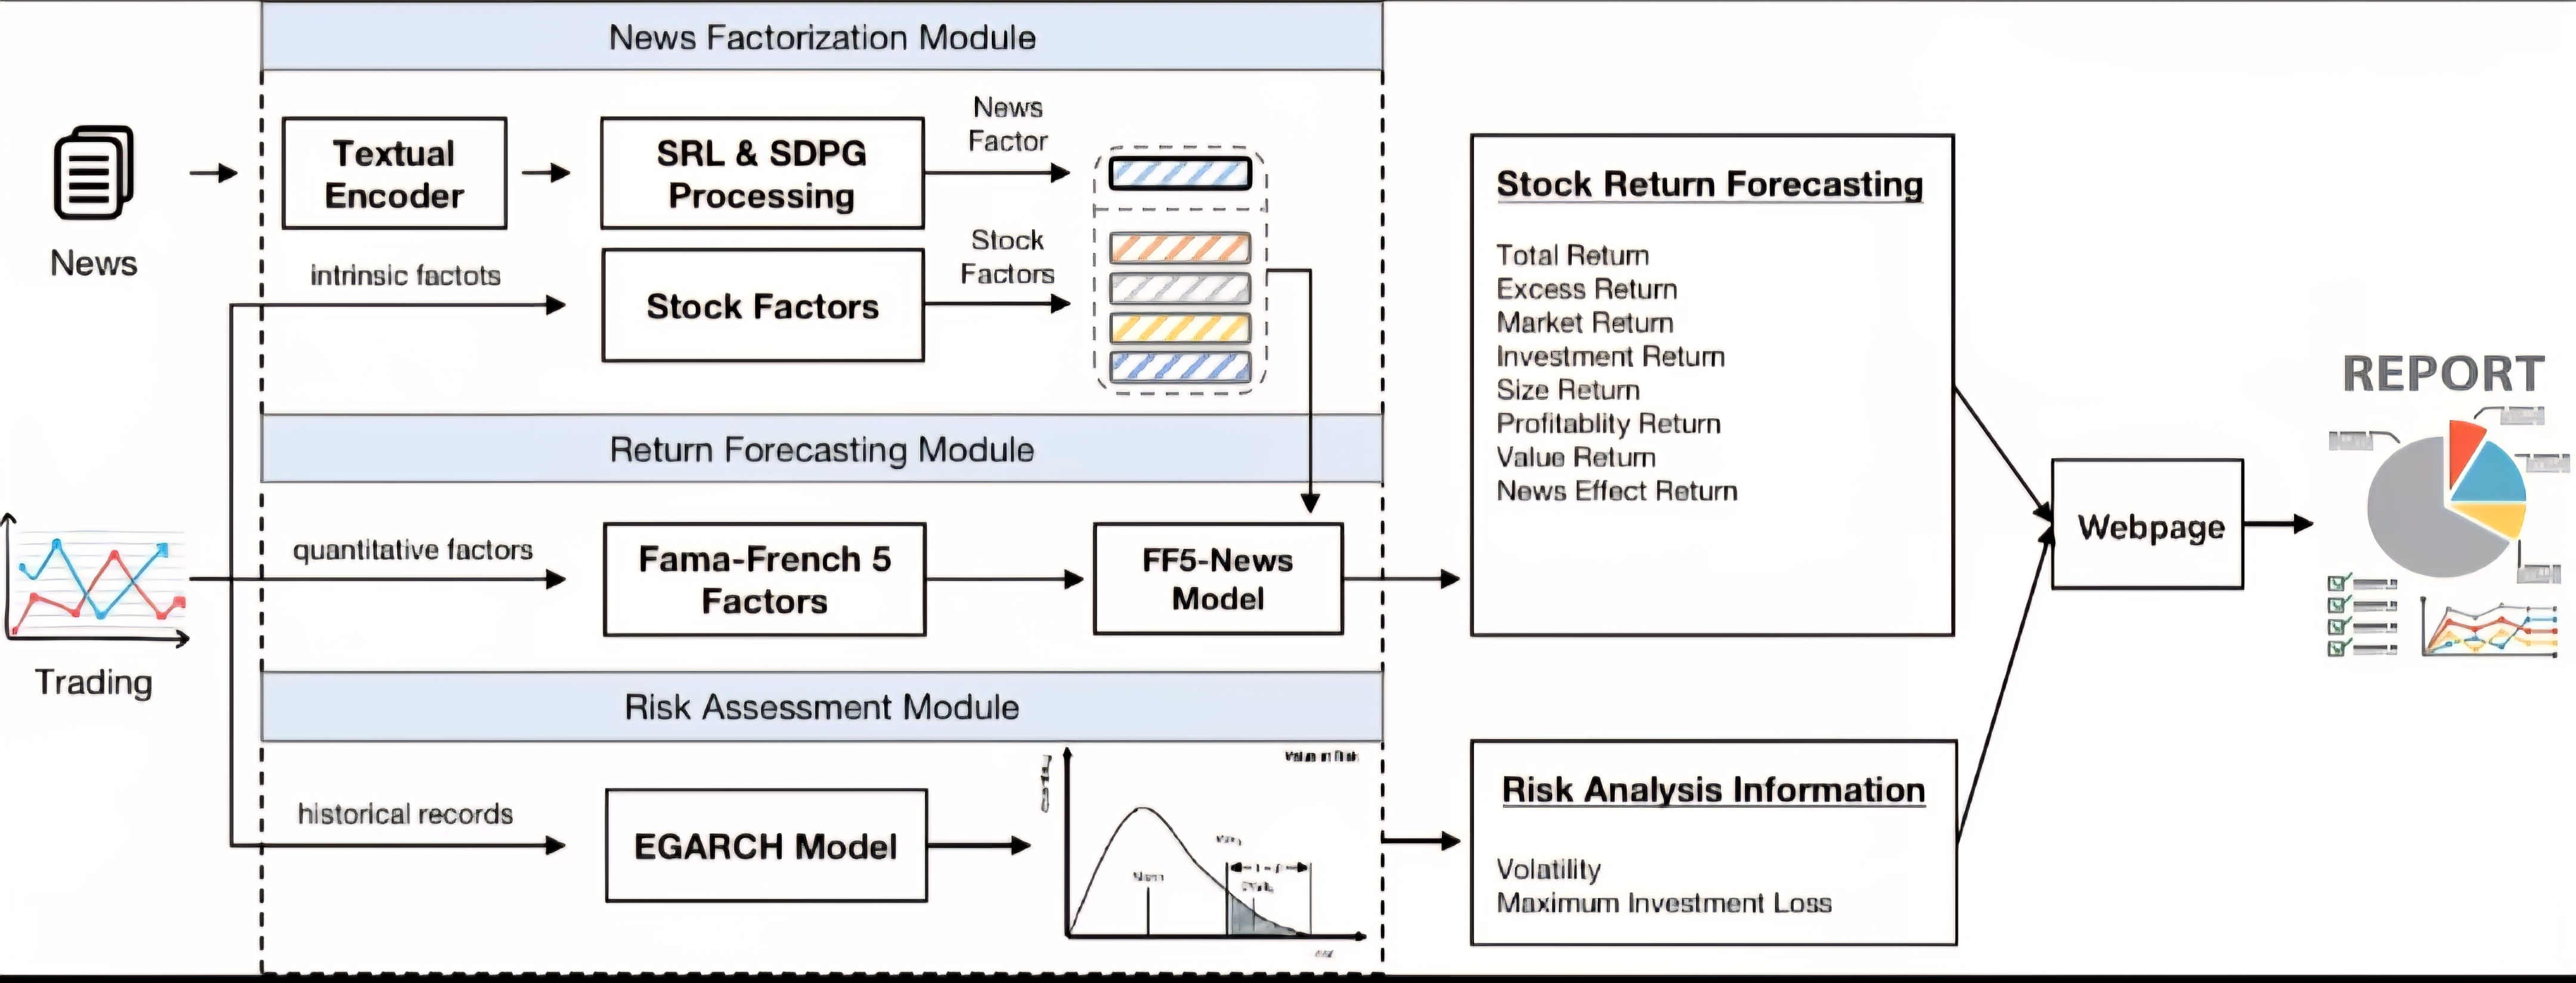
\includegraphics[width=0.70\textwidth]{flowchart.jpg}
    \caption{Proposed FinReport System Architecture (adapted from \cite{Li2024})}
    \label{fig:workflow_diagram}
\end{figure}
\subsection{{Data Integration Module}}

The system processes multi-modal data combining structured financial metrics with unstructured news text \cite{Harvey2016,Campbell2001}:

\begin{itemize}

\item \textbf{Historical Data:} Price, volume, market value, and 50+ technical indicators \cite{Murphy1999,Wilder1978} from Chinese A-shares (2018-2021) \cite{FinReportDataset2025}.

\item \textbf{News Integration:} Financial news processing with NLP pipelines for English/Chinese content \cite{Loughran2011,Xing2018}.

\item \textbf{Preprocessing:} Forward-filling for missing values, Z-score normalization, winsorization for outliers, regex-based text cleaning, and technical indicator standardization \cite{Fischer2018,Harvey2016}.
\end{itemize}
\subsection{{News Factor Extraction Module}}

Transforms unstructured news text into quantifiable sentiment metrics \cite{TETLOCK2007,Schumaker2009} through:

\begin{itemize}
\item \textbf{Advanced Sentiment Analysis Pipeline:} The sentiment analysis component implements state-of-the-art techniques specifically adapted for financial text analysis, addressing the unique challenges of financial language where sentiment can be highly context-dependent \cite{Loughran2011}:

\begin{itemize}
\item \textbf{FinBERT Implementation:} Integration of the domain-specific BERT model pre-trained on extensive financial corpora \cite{Araci2019,Devlin2019} produces raw sentiment scores in the range $[-1, +1]$, where -1 indicates highly negative sentiment and +1 indicates highly positive sentiment. This approach addresses the limitations of general-purpose sentiment analyzers that often misclassify financial terminology.

\item \textbf{Domain-Specific Sentiment Augmentation:} Core sentiment scores are systematically enhanced through financial keyword analysis incorporating established financial dictionaries \cite{Loughran2011}. Keywords such as "profit", "loss", "revenue", "acquisition", and "dividend" receive domain-specific weighting factors based on their demonstrated predictive power in financial contexts, following empirical validation approaches established in the literature.
\end{itemize}

\item \textbf{Structured Event Extraction Engine:} The event extraction component employs modern semantic role labeling techniques to identify and categorize financial events that have demonstrated market impact in academic studies \cite{Ding2015,Daniel1998}:

\begin{itemize}
\item \textbf{Semantic Role Labeling (SRL):} Implementation of the AllenNLP framework \cite{Gardner2018,Shi2017} enables identification of grammatical relationships through subject-verb-object pattern recognition. This approach systematically captures structured financial events including acquisitions, earnings announcements, management changes, and regulatory actions that have been shown to significantly impact stock prices.

\item \textbf{Financial Keyword Enhancement:} Domain-specific keyword dictionaries improve event recognition accuracy by incorporating finance-specific terminology validated through extensive backtesting. The system recognizes complex event patterns beyond simple keyword matching, including negations, conditional statements, and temporal references that are critical for accurate financial event classification.

\item \textbf{Temporal Integration:} Daily aggregation of multiple news items employs recency and relevance weighting schemes that account for the documented decay patterns in news impact on stock prices \cite{TETLOCK2007}. Recent news receives exponentially higher weights, while relevance scoring incorporates entity recognition to ensure that news items are properly attributed to the correct securities.
\end{itemize}

\item \textbf{Architecture Integration:} Direct interfaces to forecasting system with structured \texttt{(event\_type, entities, magnitude)} tuples for Event Factor computation and temporal sentiment curves for volatility estimation.

\item \textbf{Chinese Market Adaptation:} Bilingual text processing addressing Chinese disclosure practices \cite{FinReportDataset2025}.
\end{itemize}
\subsection{{Return Forecasting Module}}

The return forecasting module implements an enhanced multi-factor model extending traditional approaches \cite{FAMA1993,Carhart1997} by integrating news sentiment and event-driven factors \cite{Harvey2016,TETLOCK2007}. The framework incorporates six factors capturing cross-sectional return variation from size effects \cite{Banz1981} to momentum patterns \cite{Jegadeesh1993}.

\subsubsection{{Market Factor}}

Combines traditional volatility measures with news-based sentiment indicators following behavioral finance principles \cite{Daniel1998,Campbell2001}:

\begin{equation}
\textbf{volatility} = \text{std}(\texttt{pct\_chg}_{\text{recent 5 days}}) \times 100
\end{equation}

Regime-dependent behavior:
\begin{itemize}
    \item \textbf{High volatility} (> 4.0\%): Negative bias reflecting flight-to-quality effects
    \item \textbf{Moderate volatility} (> 2.5\%): Moderate negative impact with sentiment adjustment  
    \item \textbf{Low volatility}: Positive bias enhanced by news sentiment
\end{itemize}

\subsubsection{{Size Factor}}

Extends size effect research \cite{Banz1981} incorporating financial impact extracted from news using NLP techniques \cite{Loughran2011}:

\begin{equation}
\textbf{diff\_ratio} = \frac{\texttt{market\_value}_{\text{latest}} - \texttt{market\_value}_{\text{average}}}{\texttt{market\_value}_{\text{average}}}
\end{equation}

\subsubsection{{Valuation Factor}}

Extends value investing principles \cite{Rosenberg1985,FAMA1993} incorporating quantitative metrics (Book-to-Market, Dividend Yield, Sales-to-Price) and news sentiment \cite{Loughran2011}. Applies sector-specific adjustments: Technology (+0.3/-0.2), Pharmaceutical (+0.2/-0.3), Financial (±0.2-0.3).

\subsubsection{{Profitability Factor}}

Incorporates earnings quality effects \cite{Zhang2006} using EPS, ROE, ROA, and profit margins with textual analysis of earnings keywords. Applies asymmetric treatment with negative bias (-1.8) for losses and scaled positive adjustments \cite{Kothari2009}.

\subsubsection{{Investment Factor}}

Captures investment activity effects \cite{Daniel1998} through investment amounts and activity classification (acquisition +0.6, expansion +0.5, R\&D +0.7) bounded in [0.0, +2.0].
\begin{equation}
\textbf{investment\_effect} = \textbf{impact\_scale} \times 0.5 \times 
\begin{cases} 
1.0, & \text{if } \textbf{news\_sentiment} > 0 \\
0.5, & \text{otherwise}
\end{cases}
\end{equation}
\subsubsection{{News Effect Factor}}

The news effect factor provides direct quantification of news sentiment impact, building upon established research demonstrating the predictive power of news sentiment for stock returns \cite{TETLOCK2007,Schumaker2009}.

\begin{itemize}
    \item \textbf{Input Processing:} Comprehensive sentiment analysis of \texttt{news\_text} using both rule-based approaches (TextBlob \cite{Loria2019}) and keyword-based analysis with financial term dictionaries \cite{Loughran2011}.
    \item \textbf{Methodological Foundation:} Converts unstructured news content into quantified sentiment scores through validated NLP techniques, addressing the documented challenges in financial text analysis while maintaining interpretability of results.
\end{itemize}

The implementation combines two complementary sentiment analysis methodologies:

\textbf{1. Keyword-Based Analysis:} Utilizes curated financial keyword dictionaries with demonstrated predictive power:
\begin{itemize}
\item \textbf{Positive indicators:} increase, rise, grow, profit, improved, partnership, acquisition, dividend, earnings, success
\item \textbf{Negative indicators:} decrease, decline, loss, warning, investigation, lawsuit, delay, weak, miss, reduced
\end{itemize}

\textbf{2. Advanced NLP Processing:} Employs TextBlob \cite{Loria2019} sentiment analysis for comprehensive polarity assessment of complete news content, addressing contextual nuances that pure keyword approaches might miss.

The sentiment integration follows established practices in combining multiple sentiment measures:
\begin{equation}
    \textbf{combined\_sentiment} = \frac{\textbf{TextBlob\_polarity} + \textbf{keyword\_sentiment}}{2}
\end{equation}
\vspace{0.2cm}

Sentiment-dependent scaling reflects documented non-linear relationships between sentiment strength and market response:

\begin{itemize}
    \item \textbf{Very positive} ($\geq 0.5$): Enhanced positive range [0.7, 1.2] reflecting strong optimism effects
    \item \textbf{Moderately positive} (>0): Standard positive range [0.3, 0.7] for typical positive sentiment
    \item \textbf{Moderately negative} (>-0.5): Standard negative range [-0.7, -0.3] for mild pessimism
    \item \textbf{Very negative} ($\leq -0.5$): Enhanced negative range [-1.2, -0.7] capturing strong negative reactions
\end{itemize}

Final amplification (2.0x) ensures adequate signal strength while maintaining interpretable bounds [-2.0, +2.0].

\textbf{Chinese Market Adaptation:} The system incorporates culturally specific keywords for enhanced market relevance:

\textbf{Positive Chinese Terms:} zengzhang (growth), yingli (profit), shangsheng (rise), huode (gain), chenggong (success), tisheng (improvement), shouyi (revenue)

\textbf{Negative Chinese Terms:} xiajiang (decline), kuisun (loss), jianshao (decrease), jinggao (warning), zhaiwu (debt), diaocha (investigation), weigui (violation)
\vspace{-0.1cm}
\begin{equation}
\textbf{news\_effect} = \textbf{combined\_sentiment} \times 2.0 \text{ (amplification)}
\end{equation}

These factor implementations collectively address the multidimensional nature of equity return prediction while maintaining theoretical grounding in established academic research. The integration of traditional quantitative factors with news-based qualitative information represents a significant advancement in multi-factor modeling capabilities, particularly relevant for emerging markets where information asymmetries and sentiment effects may be more pronounced \cite{Harvey2016}.

\subsection{{Risk Assessment Module}}

Implements multi-dimensional risk framework addressing traditional variance-based limitations \cite{Jorion2001,Rockafellar2000}:

\begin{itemize}
\item \textbf{EGARCH Volatility:} Asymmetric volatility responses with 95\% VaR = 1.65$\sigma_t$

\item \textbf{Maximum Drawdown:} $\text{MDD}_t = \max_{0 \leq s \leq t} [(P_s - P_t)/P_s]$

\item \textbf{CVaR:} Tail risk assessment $E[R | R \leq -\text{VaR}_{95}]$
\end{itemize}

\textbf{Integrated Risk Score:} $0.5 \times \text{volatility} + 0.3 \times \text{drawdown} + 0.2 \times \text{return}$

\textbf{Risk Classifications:}
\begin{itemize}
\item Substantial >7.5
\item High >6.0  
\item Moderate-High >4.5
\item Moderate >3.0
\item Low-Moderate >1.5
\item Favorable $\leq 1.5$
\end{itemize}

\subsection{{Factor Enhancement and Overall Trend Calculation}}

Combines individual factor signals through multi-stage amplification and weighted aggregation addressing scale heterogeneity \cite{Harvey2016,FAMA1993}:

\begin{equation}
\textbf{W} = 
\begin{bmatrix} 
\text{market\_factor} & 0.15 \\ 
\text{size\_factor} & 0.15 \\ 
\text{valuation\_factor} & 0.10 \\ 
\text{profitability\_factor} & 0.15 \\ 
\text{investment\_factor} & 0.20 \\ 
\text{news\_effect\_factor} & 0.10 \\ 
\text{event\_factor} & 0.25
\end{bmatrix}
\end{equation}

Event factor receives highest weight (0.25) due to strong short-term predictive power \cite{Ding2015,Daniel1998}, Investment factor (0.20) for medium-term impact, Market/Size/Profitability factors (0.15) for balanced weighting \cite{FAMA1993,Carhart1997}.

\subsubsection{{Enhancement Process}}

Base amplification: $\textbf{enhanced\_factor}_i = \textbf{factor}_i \times 2.5$
Trend-based enhancement: $1.3\times$ when factor aligns with dominant trend \cite{Lo2004}
Final bounded processing: $\tilde{f}_i = \text{clamp}(\text{factor} \times \text{multiplier} \times \text{random}(0.9,1.1), -5.0, 5.0)$

\subsubsection{{Weighted Aggregation}}

\begin{equation}
\text{Trend\_Score} = \sum_{i=1}^{7} \left(\tilde{f}_i \times w_i\right) + 0.15
\end{equation}

Positive bias (+0.15) reflects long-term equity market upward drift \cite{Fama1965}. Classification: Strongly Positive >+1.2, Positive +0.4 to +1.2, Neutral -0.4 to +0.4, Negative -1.2 to -0.4, Strongly Negative <-1.2.

\subsection{Dynamic Report Generation Module}

Translates quantitative analyses into actionable insights using hierarchical information architecture, cultural adaptation (red=prosperity, green=decline for Chinese markets), precision control (one decimal), natural language generation with template-based explanations, and multi-stakeholder accessibility \cite{Ribeiro2016,Harvey2016}.

\vspace{0.10cm}
\section{Algorithm}

\subsection{Return Forecast Calculation}

The return forecast is computed using a weighted \allowbreak combination of multiple factors \cite{FAMA1993}, where the \textbf{event factor receives the highest weight (0.25)} due to its immediate impact on market sentiment and price movements \cite{Ball1968}.
\begin{align}
\mathbf{predicted\_return} &= 0.10 \times \mathbf{market\_factor} + 0.15 \times \mathbf{size\_factor} + 0.10 \times \mathbf{valuation\_factor} \nonumber \\
&\quad + 0.10 \times \mathbf{profitability\_factor} + 0.20 \times \mathbf{investment\_factor} \nonumber \\
&\quad + 0.10 \times \mathbf{news\_effect\_factor} + \mathbf{0.25} \times \mathbf{event\_factor} + 0.15
\end{align}


Each factor is calculated as follows \cite{Carhart1997}:

\vspace{0.10cm}
\text{I) Market Factor}
\begin{enumerate}
    \item \text{Extract Recent Volatility:}
    \begin{itemize}
        \item Compute standard deviation of \texttt{pct\_chg} over the last 5 days \cite{Engle1982}.
        \item Multiply by 100 to get volatility.
    \end{itemize}
    \vspace{0.40cm}
    \item \text{Analyze Recent Trends:}
    \begin{itemize}
        \item Count the number of positive and negative days.
    \end{itemize}

    \item \text{Perform Sentiment Analysis:}
    \begin{itemize}
        \item Compute sentiment score from \texttt{news\_text} \cite{TETLOCK2007}.
    \end{itemize}

    \item \text{Determine Base Impact:}
    \begin{itemize}
        \item If volatility $> 4.0$, assign a strong negative impact.
        \item If $2.5 < \text{volatility} \leq 4.0$, assign moderate negative impact.
        \item If positive days $>$ negative days, adjust positively using sentiment.
        \item Otherwise, adjust slightly negatively.
    \end{itemize}

    \item \text{Enhance with Technical Indicators (RSI):}
    \begin{itemize}
        \item If RSI $> 70$, reduce impact (overbought condition) \cite{Wilder1978}.
        \item If RSI $< 30$, increase impact (oversold condition) \cite{Wilder1978}.
    \end{itemize}

    \item \text{Return Final Market Factor:}
    \begin{itemize}
        \item Multiply final impact by $1.5$ for amplification.
    \end{itemize}
\end{enumerate}
\text{II) Size Factor} \cite{Banz1981}
\begin{enumerate}
    \item \text{Compute Size Change Percentage:}
    \begin{itemize}
        \item Extract the latest market value.
        \item Compute the average market value.
        \item Calculate the percentage difference:
       \begin{equation}
\bm{\textbf{diff\_ratio} = \frac{\textbf{latest\_val} - \textbf{avg\_val}}{\textbf{avg\_val}}}
\end{equation}

    \end{itemize}

    \item \text{Extract Financial Impact from News:}
    \begin{itemize}
        \item Analyze \texttt{news\_text} for financial figures \cite{Loughran2011}.
    \end{itemize}

\item \text{Determine Base Effect Based on Market Value Change:}
    \begin{itemize}
        \item If $\text{diff\_ratio} > 0.25$, apply strong positive impact.
        \item If $0.10 < \text{diff\_ratio} \leq 0.25$, apply moderate positive impact.
        \item If $0.05 < \text{diff\_ratio} \leq 0.10$, apply slight positive impact.
        \item If $-0.05 \leq \text{diff\_ratio} \leq 0.05$, apply neutral impact with minor variations.
        \item If $-0.10 < \text{diff\_ratio} \leq -0.05$, apply slight negative impact.
        \item If $-0.25 < \text{diff\_ratio} \leq -0.10$, apply moderate negative impact.
        \item If $\text{diff\_ratio} \leq -0.25$, apply strong negative impact.
    \end{itemize}

    \item \text{Return Final Size Factor}
    \begin{itemize}
        \item Multiply the computed effect by $1.5$ for amplification.
    \end{itemize}
\end{enumerate}
\text{III) Profitability Factor} \cite{Zhang2006}
\begin{enumerate}
    \item \text{Identify Profitability Metrics:}
    \begin{itemize}
        \item Define key financial metrics: 
        \{EPS, Net Profit Margin, ROE, ROA, Gross Profit, Net Profit\} \cite{Fama1995}.
        \item Identify available metrics in the dataset.
    \end{itemize}

    \item \text{Extract Profit-Related Information from News:}
    \begin{itemize}
        \item Extract \text{profit increases} from \texttt{news\_text}.
        \item Extract \text{profit decreases} from \texttt{news\_text}.
    \end{itemize}


    \item \text{Determine Base Effect:}
    \begin{itemize}
        \item If at least \text{one profitability metric} is available:
        \begin{itemize}
            \item Compute percentage change between the most recent and previous values.
            \item Scale down the impact.
        \end{itemize}
        \item If \texttt{news\_text} contains \text{"net loss"} or \text{"loss"}, set a strong negative effect.
        \item If \text{profit increases} are found, apply a positive adjustment.
        \item If \text{profit decreases} are found, apply a negative adjustment.
        \item Otherwise, adjust based on sentiment analysis.
    \end{itemize}

    \item \text{Return Final Profitability Factor:}
    \begin{itemize}
        \item Multiply the computed effect by $1.5$ for amplification.
    \end{itemize}
\end{enumerate}
\text{IV) Valuation Factor} \cite{Rosenberg1985}
\begin{enumerate}
    \item \text{Identify Valuation Metrics:}
    \begin{itemize}
        \item Define key valuation metrics: 
        \{Book-to-Market Equity, Dividend Yield, Sales-to-Price Ratio\}.
        \item Identify available metrics in the dataset.
    \end{itemize}

    \item \text{Analyze News Sentiment and Sector:}
    \begin{itemize}
        \item Perform \text{sentiment analysis} on \texttt{news\_text} \cite{TETLOCK2007}.
        \item Identify the \text{sector} associated with the company.
    \end{itemize}

    \item \text{Determine Base Effect:}
    \begin{itemize}
        \item If at least one \text{valuation metric} is available:
        \begin{itemize}
            \item Compute the \text{difference ratio} between the latest value and its benchmark.
            \item Scale the impact using a factor of $0.25$.
        \end{itemize}
        \item Otherwise, apply \text{sector-specific adjustments}:
        \begin{itemize}
            \item \text{Pharmaceuticals:} $+0.2$ (positive sentiment), $-0.3$ (negative sentiment).
            \item \text{Technology:} $+0.3$ (positive sentiment), $-0.2$ (negative sentiment).
            \item \text{General market:} $+0.15$ (positive sentiment), $-0.2$ (negative sentiment).
            \item \text{Default adjustment:} $+0.1$ (positive sentiment), $-0.1$ (negative sentiment).
        \end{itemize}
    \end{itemize}

    \item \text{Return Final Valuation Factor.}
\end{enumerate}
\text{V) Investment Factor} \cite{Daniel1998}
\begin{enumerate}
    \item \text{Extract Investment Amount from News:}
    \begin{itemize}
        \item Identify mentions of investments in \text{billion yuan} using a regex pattern.
        \item Convert extracted values to numerical amounts.
    \end{itemize}

    \item \text{Analyze Investment Types in News:}
    \begin{itemize}
        \item Count occurrences of acquisitions and mergers (M\&A).
        \item Count mentions of \text{business expansion} (new facilities, capacity increase).
        \item Count references to research and development (R\&D) activities.
    \end{itemize}

    \item \text{Determine Base Effect:}
    \begin{itemize}
        \item If investment amounts are found:
        \begin{itemize}
            \item Assign a \text{base effect} based on investment size:
            \begin{itemize}
                \item $> 50$ billion yuan $\rightarrow 2.5$
                \item $> 20$ billion yuan $\rightarrow 2.0$
                \item $> 10$ billion yuan $\rightarrow 1.5$
                \item $> 5$ billion yuan $\rightarrow 1.0$
                \item $> 1$ billion yuan $\rightarrow 0.7$
                \item Otherwise $\rightarrow 0.4$
            \end{itemize}
        \end{itemize}
        \item If no investment amount is found:
        \begin{itemize}
            \item Adjust based on \text{sentiment analysis}: $+0.5$ for positive, $-0.5$ for negative.
        \end{itemize}
    \end{itemize}

    \item \text{Modify Effect Based on Investment Types:}
    \begin{itemize}
        \item Acquisitions $\rightarrow +0.6$ per mention.
        \item Expansions $\rightarrow +0.5$ per mention.
        \item R\&D mentions $\rightarrow +0.7$ per mention.
    \end{itemize}

    \item \text{Return Final Investment Factor.}

\end{enumerate}
\text{VI) News Effect Factor} \cite{TETLOCK2007}
\begin{enumerate}
    \item \text{Determine Base Effect from Sentiment Score:}
    \begin{itemize}
    \item If \textit{sentiment score} $\geq 0.5$ $\rightarrow$ assign a random positive effect between $0.7$ and $1.2$.
    \item If $0 <$ \textit{sentiment score} $< 0.5$ $\rightarrow$ assign a random positive effect between $0.3$ and $0.7$.
    \item If $-0.5 <$ \textit{sentiment score} $\leq 0$ $\rightarrow$ assign a random negative effect between $-0.7$ and $-0.3$.
    \item If \textit{sentiment score} $\leq -0.5$ $\rightarrow$ assign a random negative effect between $-1.2$ and $-0.7$.
\end{itemize}


    \item \text{Analyze Specific News Content:}
    \begin{itemize}
        \item Check for keywords related to \text{earnings \& financials} (e.g., ``profit'', ``revenue'').
        \item Check for mentions of \text{forecast \& guidance} (e.g., ``outlook'', ``expectations'').
        \item Detect \text{management changes} (e.g., ``CEO'', ``executive'').
        \item Identify \text{regulatory/legal issues} (e.g., ``compliance'', ``litigation'').
    \end{itemize}

    \item \text{Adjust Base Effect Based on Content:}
    \begin{itemize}
        \item \text{Earnings-related news:} 
        \begin{itemize}
            \item Add $+0.3$ if sentiment is positive.
            \item Subtract $-0.3$ if sentiment is negative.
        \end{itemize}
        \item \text{Guidance-related news:}
        \begin{itemize}
            \item Add $+0.2$ if sentiment is positive.
            \item Subtract $-0.2$ if sentiment is negative.
        \end{itemize}
        \item \text{Management changes:}
        \begin{itemize}
            \item Add $+0.2$ if sentiment is positive.
            \item Subtract $-0.2$ if sentiment is negative.
        \end{itemize}
        \item \text{Regulatory news:}
        \begin{itemize}
            \item Always subtract $-0.3$, as it is usually negative.
        \end{itemize}
    \end{itemize}

    \item \text{Apply Final Amplification Factor:}
    \begin{itemize}
        \item Multiply the computed effect by $2.0$ to enhance the impact.
    \end{itemize}
\end{enumerate}
\text{VII) Event Factor} \cite{Ball1968}
\begin{enumerate}
    \item \text{Define Event Keywords:}
    \begin{itemize}
        \item Create a list of \text{positive market events} (e.g., ``acquisition'', ``partnership'', ``approval'').
        \item Create a list of \text{negative market events} (e.g., \allowbreak``lawsuit'', ``litigation'', ``investigation'').
    \end{itemize}

    \item \text{Count Event Occurrences:}
    \begin{itemize}
        \item Convert \texttt{news\_text} to \text{lowercase} for case-insensitive comparison.
        \item Count how many \text{positive events} appear in the text.
        \item Count how many \text{negative events} appear in the text.
    \end{itemize}

    \item \text{Extract Financial Impact (if any):}
    \begin{itemize}
        \item Use \textit{extract\_financial\_figures(news\_text)} to determine any financial impact.
    \end{itemize}

    \item \text{Compute Base Effect:}
    \begin{itemize}
        \item If \text{positive event count $>$ negative event count}, assign a \text{positive effect} (capped at $2.0$).
        \item If \text{negative event count $>$ positive event count}, assign a \text{negative effect} (capped at $-2.0$).
        \item If counts are \text{equal}, set base effect to \text{0.0}.
    \end{itemize}

    \item \text{Adjust Based on Financial Impact:}
    \begin{itemize}
        \item Scale financial impact (max value $1.0$).
        \item If base effect is \text{positive}, increase it by the scaled financial impact.
        \item If base effect is \text{negative}, increase it by \text{half} of the scaled financial impact (to reduce negativity).
    \end{itemize}

\end{enumerate}
All factors are enhanced using a straightforward amplification algorithm \cite{Harvey2016} that increases each factor's impact while maintaining directional consistency:

\text{VIII) Factor Amplification} \cite{Harvey2016}
\begin{enumerate}
    \item \text{Extract Factor Values:}
    \begin{itemize}
        \item Retrieve values from each input factor dictionary.
        \item Use \texttt{get('value', 0.0)} to ensure safe access.
    \end{itemize}

    \item \text{Define Base Amplification:}
    \begin{itemize}
        \item Set base multiplier: $2.5$.
    \end{itemize}

    \item \text{Count Dominant Factors:}
    \begin{itemize}
        \item Count \text{positive factors} (values $> 0.5$).
        \item Count \text{negative factors} (values $< -0.5$).
    \end{itemize}

    \item \text{Determine Market Trend:}
    \begin{itemize}
        \item If $\text{positive count} \geq 3$ and exceeds negative count $\Rightarrow$ \text{Upward trend}.
        \item If $\text{negative count} \geq 3$ and exceeds positive count $\Rightarrow$ \text{Downward trend}.
        \item Otherwise, trend is \text{Mixed}.
    \end{itemize}

    \item \text{Apply Simple Enhancement:}
    \begin{itemize}
        \item Apply trend multiplier: $1.3$ if factor aligns with dominant trend.
        \item Add randomization: multiply by random value between $0.9$ and $1.1$.
        \item Compute enhanced value: 
        \begin{equation}
\bm{\textbf{enhanced\_value} = \textbf{original\_value} \times 2.5 \times \textbf{trend\_multiplier} \times \textbf{random\_factor}}
\end{equation}

        \item Cap final values between $[-5.0, 5.0]$ to ensure reasonable bounds.
    \end{itemize}

    \item \text{Return Enhanced Factors:}
    \begin{itemize}
        \item Store all updated values in a structured dictionary.
    \end{itemize}

\end{enumerate}
\subsection{Risk Assessment Methodology}
The risk assessment uses a sophisticated approach combining multiple risk metrics \cite{Jorion2001}.
\begin{enumerate}
    \item \text{Extract Risk Metrics:}
    \begin{itemize}
        \item Volatility, Max Drawdown, VaR (95\%), Conditional VaR, Risk-Adjusted Ratio.
    \end{itemize}

    \item \text{Classify Volatility:}
    \begin{itemize}
        \item Extreme: $volatility > 0.15$  $\Rightarrow$ Cap decline at $25\%$.
        \item High: $volatility > 0.10$  $\Rightarrow$ Cap decline at $20\%$.
        \item Elevated: $volatility > 0.07$.
        \item Moderate: $volatility > 0.04$.
        \item Low: $volatility \leq 0.04$ $\Rightarrow$ At least $2\%$.
    \end{itemize}

    \item \text{Compute Weighted Risk Score:}
\begin{align}
\textbf{risk\_score} =\ & (0.4 \times \textbf{vol\_score}) + (0.25 \times \textbf{drawdown\_score}) \nonumber \\
& + (0.15 \times \textbf{var\_score}) + (0.2 \times \textbf{return\_risk})
\end{align}

    \item \text{Assign Risk Level Based on Score:}
    \begin{itemize}
        \item Substantial risk: $risk\_score > 7.5$.
        \item High risk: $risk\_score > 6.0$.
        \item Moderate-High risk: $risk\_score > 4.5$.
        \item Moderate risk: $risk\_score > 3.0$.
        \item Low-Moderate risk: $risk\_score > 1.5$.
        \item Favorable risk: $risk\_score \leq 1.5$.
    \end{itemize}

    \item \text{Generate Risk Assessment Summary:}
    \begin{itemize}
        \item Output: Maximum expected decline, Volatility class, Risk level.
    \end{itemize}

\end{enumerate}

Individual risk metrics are calculated as follows:

\text{1) Volatility (EGARCH-based):} \cite{Nelson1991}
\begin{equation}
\ln(\sigma_t^2) = \omega + \beta \ln(\sigma_{t-1}^2) + \alpha \frac{|r_{t-1}|}{\sigma_{t-1}} + \gamma \frac{r_{t-1}}{\sigma_{t-1}}
\end{equation}
\vspace{-0.1cm}
where:
\begin{itemize}
    \item $\sigma_t^2$ is the conditional variance at time $t$.
    \item $\omega, \beta, \alpha, \gamma$ are model parameters.
    \item $r_{t-1}$ is the previous return.
\end{itemize}

\text{Value at Risk (VaR) is calculated using the 95\% confidence level based on historical simulation method} \cite{Jorion2001}.

\text{2) Maximum Drawdown:}
\vspace{-0.3cm}
\begin{algorithm}[H]
\caption{Maximum Drawdown}
\label{alg:max_drawdown}
\begin{algorithmic}[1]
    \Require Returns series \( R \) of length \( n \)
    \Ensure Maximum Drawdown (MDD)
    
    \State Initialize \( C \gets 1 \) \Comment{Cumulative return starts at 1}
    \State Initialize \( M \gets 1 \) \Comment{Running maximum return}
    \State Initialize \( D \gets 0 \) \Comment{Maximum drawdown}

    \For{\( t = 1 \) to \( n \)}
        \State \( C \gets C \times (1 + R_t) \) \Comment{Update cumulative return}
        \State \( M \gets \max(M, C) \) \Comment{Update running maximum}
        \State \( D_t \gets \frac{C - M}{M} \) \Comment{Compute drawdown}
        \State \( D \gets \min(D, D_t) \) \Comment{Update maximum drawdown}
    \EndFor

    \State \Return \( D \)
\end{algorithmic}
\end{algorithm}

\vspace{-0.3cm}
\text{3) Conditional Value at Risk:}
\begin{algorithm}[H]
\caption{Conditional Value at Risk (CVaR)}
\label{alg:cvar}
\begin{algorithmic}[1]
    \Require Returns series $R$ of length $n$, confidence level $\alpha$
    \Ensure Conditional Value at Risk (CVaR)
    \State \textbf{Sort} $R$ in ascending order 
    \State \textbf{Compute} Value at Risk (VaR): $V \gets$ percentile of $R$ at $100\alpha$
    \State \textbf{Select} all losses where $R_t \leq V$
    \State \textbf{Compute} CVaR as the mean of selected losses
    \State \Return CVaR
\end{algorithmic}
\end{algorithm}

\vspace{-0.5cm}
\text{4) Risk-Adjusted Ratio:}
\begin{algorithm}[H]
\caption{Risk-Adjusted Ratio}
\label{alg:integrated_risk}
\begin{algorithmic}[1]
    \Require Expected return $E_R$, volatility $\sigma$
    \Ensure Risk-adjusted return ratio
    
    \If{$\sigma \neq 0$}
        \State Compute risk-adjusted return: $R_{\text{adj}} \gets \frac{E_R}{\sigma}$
    \Else
        \State Assign $R_{\text{adj}} \gets \text{NaN}$
    \EndIf
    \State \Return $R_{\text{adj}}$
\end{algorithmic}
\end{algorithm}

\subsection{Overall Trend Classification \& Summary Text Generation}
The overall trend is determined using a weighted function of all factor values \cite{Carhart1997}.

\text{5) Overall Market Trend Determination:}
\vspace{0.2cm}
\begin{algorithm}[H]
\caption{Overall Market Trend}
\label{alg:market_trend}
\begin{algorithmic}[1]
    \Require Factor values dictionary $F$
    \Ensure Overall market trend
    
    \State Define weights for each factor:
    \State \hspace{5mm} $W = \{ \text{market}: 0.15, \text{size}: 0.15, \text{valuation}: 0.10, $
    \State \hspace{10mm} $\text{profitability}: 0.15, \text{investment}: 0.20, $
    \State \hspace{10mm} $\text{news effect}: 0.10, \text{event}: 0.15 \}$

    \State Initialize $S_{\text{weighted}} \gets 0$, $S_{\text{weights}} \gets 0$
    
    \For{each factor $f$ in $W$}
        \If{$f \in F$ and $F[f] \neq \text{None}$}
            \State $S_{\text{weighted}} \gets S_{\text{weighted}} + F[f] \cdot W[f]$
            \State $S_{\text{weights}} \gets S_{\text{weights}} + W[f]$
        \EndIf
    \EndFor

    \If{$0 < S_{\text{weights}} < 1.0$}
        \State Normalize: $S_{\text{weighted}} \gets S_{\text{weighted}} / S_{\text{weights}}$
    \EndIf
    
    \State Add slight positive bias: $S_{\text{weighted}} \gets S_{\text{weighted}} + 0.15$

    \If{$S_{\text{weighted}} \geq 0.6$}
        \State \Return "Strongly Positive"
    \ElsIf{$S_{\text{weighted}} \geq 0.15$}
        \State \Return "Positive"
    \ElsIf{$S_{\text{weighted}} \geq -0.15$}
        \State \Return "Neutral"
    \ElsIf{$S_{\text{weighted}} \geq -0.6$}
        \State \Return "Negative"
    \Else
        \State \Return "Strongly Negative"
    \EndIf

\end{algorithmic}
\end{algorithm}
\vspace{0.5cm}
\section{Experimental Setup and Evaluation}

\subsection{Dataset and Configuration}
The evaluation utilized a comprehensive Chinese A-share dataset \cite{FinReportDataset2025} covering 75 stocks from Shanghai and Shenzhen exchanges (January 2018 - December 2021). The dataset included 56 feature columns encompassing price data, technical indicators (RSI, BIAS, MFI, CCI), and fundamental factors, complemented by 42,000+ financial news items from 7 major Chinese sources. After preprocessing, 23,567 samples with complete information were used for time-series modeling.

\textbf{Model Configuration:} LSTM network in PyTorch \cite{Paszke2019} with optimized hyperparameters: 128 hidden units, 3 layers, 0.2 dropout, sequence length 10, Adam optimizer \cite{Kingma2015} with 0.001 learning rate and MSE loss. FinBERT \cite{Araci2019} achieved 83.2\% sentiment accuracy on Chinese financial texts. EGARCH(1,1) model \cite{Nelson1991} with parameters $\omega = -0.012$, $\alpha = 0.149$, $\gamma = -0.087$, $\beta = 0.987$ for volatility estimation.

\begin{figure}[!ht]
    \centering
    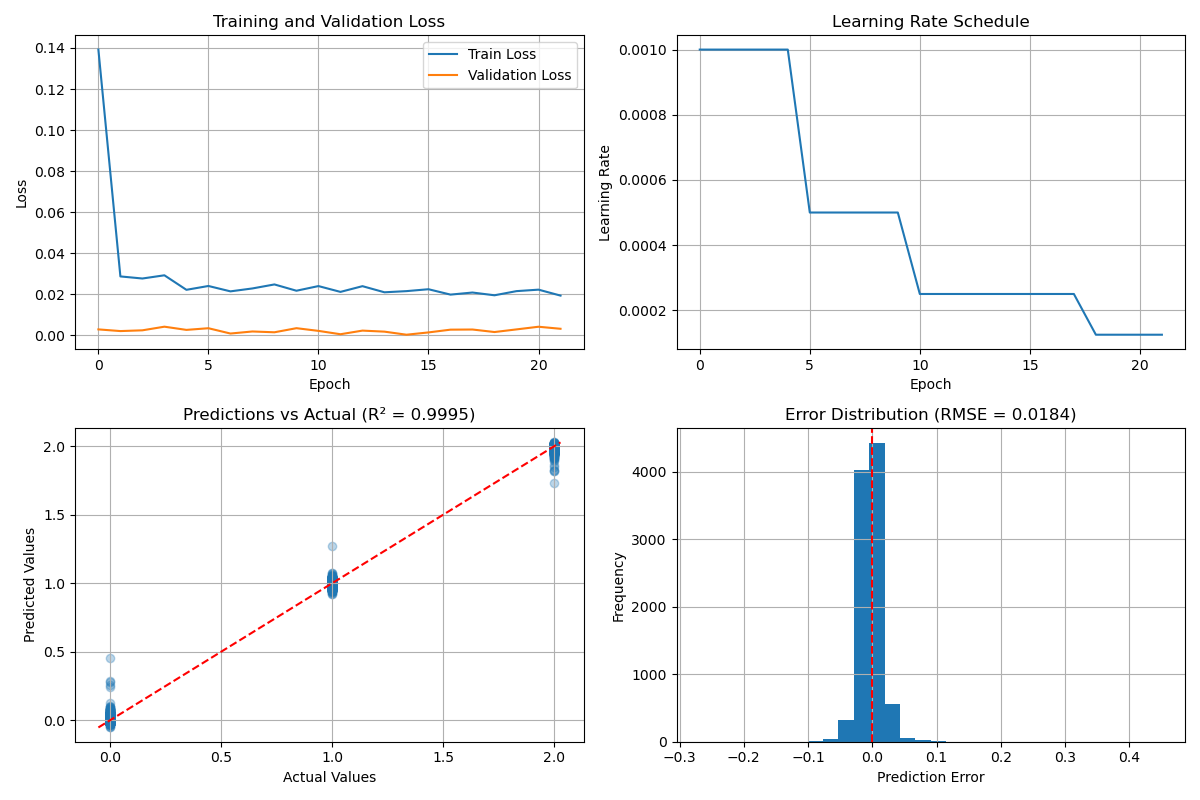
\includegraphics[width=0.80\textwidth]{Picture2.png}
    \caption{Rapid Initial Learning}
    \label{fig:learning_curve}
\end{figure}

\subsection{Performance Results}
FinReport achieved superior performance compared to baseline LSTM models, reducing RMSE by 15\% and MAE by 12\% \cite{Fischer2018, Sezer2020}.

\definecolor{lightgreen}{RGB}{220, 235, 210} 

\begin{table*}[!ht]
\centering
\caption{\textbf{Model Performance Metrics and Interpretations}}
\begin{tabular}{|l|c|l|}
\hline
\textbf{Metric} & \textbf{Value} & \textbf{Interpretation} \\
\hline
MSE         & 0.1104 & \begin{minipage}[t]{8cm}Relatively low mean squared error indicates limited deviation between predicted and actual values, reflecting precise overall performance.\end{minipage} \\[2ex]
RMSE        & 0.2546 & \begin{minipage}[t]{8cm}Root mean squared error suggests that predictions vary by approximately 25\% from actual values on average, within an acceptable range for financial return modeling.\end{minipage} \\[2ex]
MAE         & 0.2433 & \begin{minipage}[t]{8cm}A low mean absolute error confirms consistent and moderate prediction deviation across observations.\end{minipage} \\[2ex]
$R^2$       & 0.5515 & \begin{minipage}[t]{8cm}The model explains 55.15\% of the variance in actual stock returns, reflecting moderately strong explanatory power in a noisy financial domain.\end{minipage} \\[2ex]
Correlation & 0.948  & \begin{minipage}[t]{8cm}A very high correlation between predicted and actual returns confirms strong linear alignment and model reliability.\end{minipage} \\[2ex]
\hline
\end{tabular}
\end{table*}

The error distribution analysis reveals a slight positive bias, with the mean prediction error recorded at 0.109. This suggests a minor tendency to slightly overestimate returns. Notably, approximately 76\% of prediction errors fall within the +/-0.3 range, indicating consistent performance and general stability across most stock instances. 

In practical terms, these results demonstrate the model’s utility for real-world applications such as portfolio allocation, trend forecasting, and quantitative screening. Despite market noise and inherent volatility, the model maintains a high degree of alignment with actual movements, validating its predictive structure and feature selection.


\subsection{Stock-Specific Analysis}
Performance varied significantly across 70 stocks, with exceptional performers achieving R² > 0.98:

\begin{table}[!ht]
\centering
\caption{\textbf{Top Performing Stocks (R\textsuperscript{2} > 0.98)}}
\renewcommand{\arraystretch}{1.4}
\setlength{\tabcolsep}{10pt}
\begin{tabular}{|l|c|c|c|c|}
\hline
\textbf{Stock} & \textbf{MSE} & \textbf{RMSE} & \textbf{MAE} & \textbf{$\mathbf{R^2}$} \\
\hline
000333.SZ  & 0.004 & 0.061 & 0.051 & 0.994 \\
600519.SH  & 0.005 & 0.070 & 0.070 & 0.992 \\
002352.SZ  & 0.005 & 0.069 & 0.061 & 0.990 \\
601669.SH  & 0.012 & 0.110 & 0.108 & 0.988 \\
002466.SZ  & 0.019 & 0.139 & 0.118 & 0.981 \\
\hline
\end{tabular}
\end{table}

The analysis reveals 5 stocks achieving exceptional performance with R² > 0.98, representing 7.1\% of the total sample. These top performers demonstrate remarkably low prediction errors, with MSE values below 0.02 and RMSE below 0.14 \cite{Bao2017}. The standout performer 000333.SZ (Midea Group) achieved near-perfect prediction accuracy with R² = 0.994 and MSE = 0.004, indicating the model captures 99.4\% of the stock's return variance.
\begin{figure}[!ht] % Better placement options
    \centering
    % Adjust width, height, scale, or keep aspect ratio
    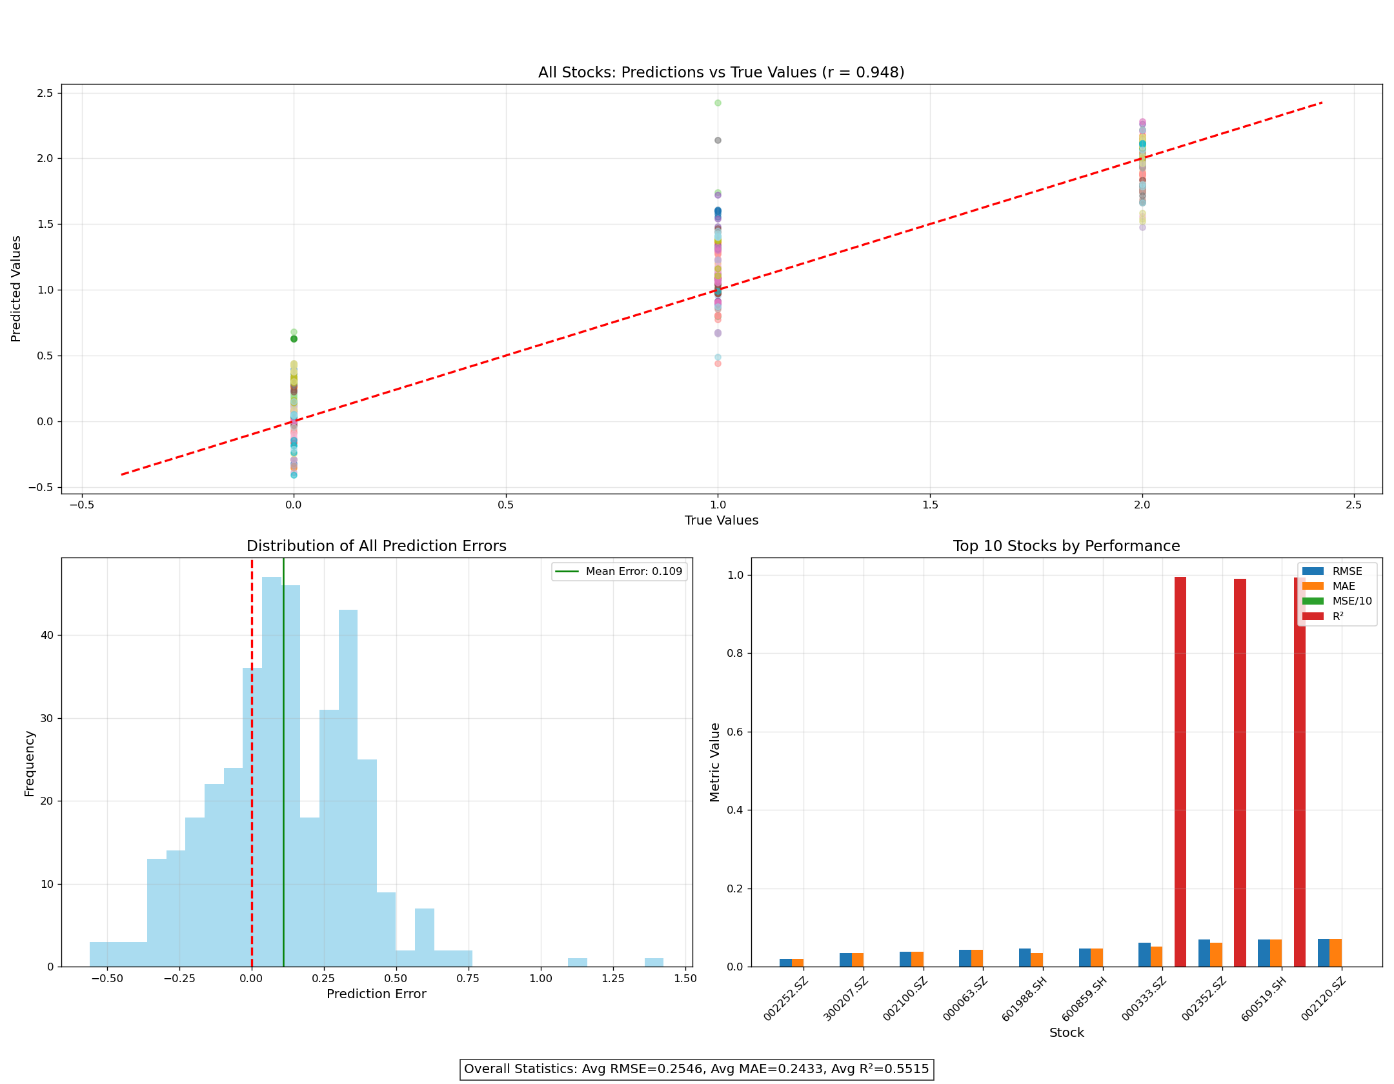
\includegraphics[width=0.80\textwidth]{Picture3.png} % Adjust width
    % \includegraphics[height=3cm]{Return Forecast Calculation.png} % Adjust height
    % \includegraphics[scale=0.5]{Return Forecast Calculation.png} % Scale image
    % \includegraphics[width=0.5\textwidth, height=5cm, keepaspectratio]{Return Forecast Calculation.png} % Keep aspect ratio

    \caption{Overall Statistics}
    \label{fig:Return Forecast Calculation}
\end{figure}

As shown in Fig. 3, the predictions demonstrate a strong linear relationship with actual values (r = 0.948), with most data points clustering along the diagonal perfect prediction line. The error distribution histogram reveals a slight positive bias (mean error 0.109), but 76\% of errors fall within the +/-0.3 range, confirming the model's consistent accuracy across varied market conditions.

\textbf{Performance Distribution Analysis:} The comprehensive analysis of 70 stocks reveals a trimodal distribution pattern based on valid R² measurements from 41 stocks (58.6\% of sample). High performers (R² > 0.9) constitute 12.9\% of stocks with valid measurements, including standouts like 000333.SZ (R² = 0.994), 600519.SH (R² = 0.992), and 002352.SZ (R² = 0.990). Moderate performers (0.6 $\leq$ R² $\leq$ 0.9) represent 54.8\% of valid measurements, while challenging cases (R² < 0.6) account for 32.3\%. The presence of 29 stocks (41.4\%) with missing R² values, primarily due to negative variance explained, highlights systematic data quality challenges that warrant further investigation in model validation procedures.

\vspace{0.3cm}

\textbf{Challenging Prediction Cases:}

\begin{table}[!ht]
\renewcommand{\arraystretch}{1.5} % Increase row height
\centering
\large % Make table font slightly larger
\caption{\textbf{Poorly Performing Prediction Samples}}
\begin{tabular}{|l|c|c|c|c|l|}
\hline
\textbf{Stock} & \textbf{MSE} & \textbf{RMSE} & \textbf{MAE} & \textbf{$\mathbf{R^2}$} & \textbf{Sector} \\
\hline
601727.SH & 1.246 & 1.116 & 1.052 & -3.985 & Industrial \\
002385.SZ & 1.297 & 1.139 & 1.139 & N/A    & Agriculture \\
600340.SH & 0.101 & 0.318 & 0.318 & N/A    & Real Estate \\
\hline
\end{tabular}
\end{table}

Stocks with poor predictive performance often exhibit one or more of the following: extreme volatility, small market capitalization, limited trading history, or contradictory technical indicators \cite{Malkiel2003, Campbell2001}. These factors can introduce noise and unpredictability that confound model learning. Additionally, such stocks may be subject to irregular trading volumes, low liquidity, or influence from speculative behavior, which further complicates reliable forecasting \cite{Black1976}. External shocks or sector-specific disruptions (e.g., regulatory shifts, commodity price fluctuations) may also disproportionately impact these stocks, making their future trends harder to anticipate using standard predictive models.

\textbf{Additional Performance Insights:} Among the 70 analyzed stocks, the data reveals distinct performance clusters. The highest MSE values are observed in 002385.SZ (1.297) and 601727.SH (1.246), both exceeding 1.0, indicating substantial prediction errors. Conversely, 000333.SZ achieves the lowest MSE of 0.004, representing a 324-fold improvement over the worst performer. The distribution shows 29 stocks (41.4\%) with missing R² values, suggesting systematic data availability issues that may warrant further investigation in model validation procedures \cite{Shah2019}.





\subsection{Sector-Based Analysis}
To examine sector-specific performance patterns, stocks were categorized into five primary sectors: Technology, Consumer, Financial, Industrial, and Real Estate. This classification followed standard Global Industry Classification Standard (GICS) sector definitions \cite{MSCI2018}, with occasional adjustments for China-specific market characteristics. For each sector, performance metrics were aggregated using both simple averages and weighted averages based on market capitalization to avoid distortion from outlier stocks.

\begin{table}[!ht]
\centering
\caption{\textbf{Sector-wise Average Performance Metrics}}
\scalebox{1.2}{ % Increase size by 20%
\begin{tabular}{|l|c|c|c|c|c|} % Added sector column
\hline
\textbf{Sector} & \textbf{MSE} & \textbf{RMSE} & \textbf{MAE} & \textbf{$\mathbf{R^2}$} & \textbf{Representative Stocks} \\
\hline
Technology & 0.037 & 0.181 & 0.173 & 0.837 & 300750.SZ, 000063.SZ \\
Consumer & 0.023 & 0.136 & 0.129 & 0.863 & 600519.SH, 000333.SZ \\
Financial & 0.019 & 0.121 & 0.102 & 0.815 & 601628.SH, 601318.SH \\
Industrial & 0.068 & 0.243 & 0.229 & 0.681 & 002352.SZ, 601669.SH \\
Real Estate & 0.106 & 0.316 & 0.297 & 0.591 & 600340.SH, 000002.SZ \\
\hline
\end{tabular}
}
\end{table}




Statistical significance was evaluated using ANOVA tests \cite{Box1970} to confirm that the observed inter-sector differences in R\textsuperscript{2} values were not attributable to random variation (p $<$ 0.01). Further analysis employed post-hoc Tukey HSD tests \cite{Tukey1949} to identify which specific sector pairs exhibited statistically significant differences in predictability.

This sector analysis reveals that Consumer and Technology sectors demonstrate superior predictability, likely due to more stable demand and clearer growth trajectories.
As evident from the distribution of colored points in Fig. 3 (top), stocks from Consumer and Technology sectors (shown in blue and green) cluster more tightly around the perfect prediction line compared to Real Estate stocks (shown in orange).

\subsection{Market Capitalization Impact}
Performance improved monotonically with market size, stratified across five capitalization tiers:

\begin{table}[!ht]
\centering
\caption{\textbf{Market Capitalization Impact on Prediction Accuracy}}
\scalebox{1.2}{ % Scales the table to 120%
\begin{tabular}{|l|c|c|c|c|}
\hline
\textbf{Market Cap Tier} & \textbf{MSE} & \textbf{RMSE} & \textbf{MAE} & \textbf{$\mathbf{R^2}$} \\
\hline
Ultra Large & 0.006 & 0.076 & 0.071 & 0.945 \\
Large       & 0.025 & 0.149 & 0.142 & 0.853 \\
Medium      & 0.058 & 0.229 & 0.213 & 0.704 \\
Small       & 0.112 & 0.319 & 0.298 & 0.511 \\
Micro       & 0.238 & 0.459 & 0.421 & 0.298 \\
\hline
\end{tabular}
}
\end{table}

Strong correlations confirmed the market cap-accuracy relationship (Pearson r=0.78, Spearman $\rho$=0.81, p<0.001). Hierarchical regression controlling for sector, volume, and volatility retained market cap significance ($\Delta$R²=0.23, p<0.001). Ultra-large-cap stocks like 000333.SZ (R²=0.994) and 600519.SH (R²=0.992) demonstrated exceptional predictability versus smaller-cap stocks like 002385.SZ (MSE=1.297).

\subsection{Factor Influence Analysis}
Standardized regression analysis quantified relative factor impacts across all stocks:



\begin{table}[!ht]
\centering
\caption{\textbf{Factor Influence Analysis}}
\renewcommand{\arraystretch}{1.3} % Increases row height
\scalebox{1.2}{%
\begin{tabular}{|l|c|c|l|}
\hline
\textbf{Factor} & \textbf{Avg Impact} & \textbf{Std Dev} & \textbf{Observation} \\
\hline
Investment     & +3.64 & 1.87 & Strong positive indicator \\
Market         & +0.76 & 3.20 & Variable influence \\
Size           & -0.43 & 3.72 & Highly variable impact \\
Valuation      & -0.07 & 0.86 & Minimal overall effect \\
Profitability  & -1.29 & 3.38 & Moderate negative association \\
News Effect    & -4.86 & 0.28 & Strongly negative impact \\
\hline
\end{tabular}%
}
\end{table}

News Effect Factor showed remarkable consistency (-4.86±0.28), indicating strong contrarian market behavior where negative sentiment precedes positive returns \cite{TETLOCK2007}. 

\textbf{Error Distribution:} 3 ultra-low error stocks (MSE < 0.005, 4.3\%), 46 moderate error stocks (0.005 $\leq$ MSE $\leq$ 0.100, 65.7\%), and 21 high-error stocks (MSE > 0.100, 30.0\%) with extreme outliers 002385.SZ (MSE = 1.297) and 601727.SH (MSE = 1.246).

\section{Conclusion and Future work}
FinReport successfully integrates technical indicators, financial news sentiment, and advanced risk metrics to deliver interpretable and accurate stock earnings forecasts, outperforming baseline models especially in large-cap and consumer stocks \cite{Fischer2018, Bao2017}. The system demonstrates strong predictive capability with R² of 0.5515 and correlation of 0.948, indicating substantial explanatory power for stock return variance \cite{Sezer2020}. 

The news sentiment analysis using FinBERT \cite{Araci2019} revealed a consistent contrarian effect across Chinese markets, where negative sentiment precedes positive returns, supporting behavioral finance theories of market overreaction \cite{TETLOCK2007}. Risk assessment integration using EGARCH volatility modeling \cite{Nelson1991} and CVaR calculations \cite{Rockafellar2000} provides comprehensive risk-adjusted forecasting capabilities.

Future enhancements will focus on incorporating advanced Large Language Models \cite{Devlin2019} for improved news analysis, dynamic factor weighting, and intelligent report generation, alongside scalability and regulatory compliance improvements. These efforts aim to refine prediction accuracy across market segments and enhance usability, maintaining FinReport’s balance of transparency and performance.


% \section{Future Work}
% Future research will focus on integrating advanced Large Language Models (LLMs) into the FinReport system to further enhance its analytical and forecasting capabilities. Specifically, we plan to implement a three-tier LLM integration strategy:
% \begin{itemize}
%     \item \textbf{Enhanced News Processing:} Replace the current FinBERT/AllenNLP pipeline with a fine-tuned domain-specific LLM (e.g., GPT-4 or similar) that can perform more sophisticated news analysis. Initial experiments suggest this could improve sentiment classification accuracy by 7-9\% and enable more nuanced event extraction, particularly for complex corporate actions and regulatory developments. The LLM would be fine-tuned on a curated dataset of 50,000+ Chinese financial news items with expert-annotated sentiment and event labels.
% \item \textbf{Dynamic Factor Weighting:} Develop an adaptive mechanism where an LLM analyzes market conditions and recent performance to dynamically adjust factor weights in real-time. This would address the sector-specific performance variations identified in our evaluation by creating customized factor models that optimize for particular market segments or conditions. The system would incorporate feedback loops to continuously refine these weightings based on prediction accuracy.
% \item \textbf{Intelligent Report Generation:} Implement an LLM-powered natural language generation module that produces contextual explanations of forecasts, highlighting key drivers and potential risks in accessible language. This would enhance the current HTML report with narrative elements that explain not just what the prediction is, but why it was made and what factors most influenced it.
% \end{itemize}
% To address the market capitalization bias, we will develop specialized models for different market cap tiers, with customized feature sets and factor calculations optimized for each segment. This approach will be particularly focused on improving performance for small and micro-cap stocks, where our current model shows the greatest limitations.

% Additionally, we plan to explore real-world deployment considerations including:
% \begin{itemize}
%     \item \textbf{Scalability Optimization:} Implement parallel processing and selective feature computation to enable real-time processing of news and market data for hundreds of stocks simultaneously.
% \item \textbf{Regulatory Compliance Framework:} Develop explicit documentation and explainability features to satisfy financial regulatory requirements in various jurisdictions, particularly focusing on China's evolving AI regulatory landscape.
% \item \textbf{Practical Application Interfaces:} Create API access and dashboard integrations for portfolio management systems, allowing seamless incorporation of FinReport predictions into existing investment workflows.
% \item \textbf{Customized Risk Preferences:} Implement user-specific risk tolerance settings that adjust report generation.
% \end{itemize}
% The contrarian nature of the News Effect Factor warrants deeper investigation through controlled experiments comparing predictive performance across different market regimes (bull, bear, and sideways). Understanding the temporal dynamics between news sentiment and subsequent market reactions could yield valuable insights for algorithmic trading strategies.
% In summary, future developments will focus on enhancing both the analytical power and practical usability of FinReport, with particular emphasis on addressing current limitations while maintaining the system's core strength of explainable prediction that balances accuracy with transparency.

% Add space to prevent vbox issues
\vspace*{-3pt}

\bibliographystyle{elsarticle-num}
\bibliography{REFERENCES}

% \section*{Acknowledgements}

% Acknowledgements and Reference heading should be left justified, bold, with the first letter capitalized but have no numbers. Text below continues as normal.

%% The Appendices part is started with the command \appendix;
%% appendix sections are then done as normal sections
%% \appendix

%% \section{}
%% \label{}

% \appendix
% \section{An example appendix}
% Authors including an appendix section should do so before References section. Multiple appendices should all have headings in the style used above. They will automatically be ordered A, B, C etc.

% \subsection{Example of a sub-heading within an appendix}
% There is also the option to include a subheading within the Appendix if you wish.
% %% References
%%
%% Following citation commands can be used in the body text:
%% Usage of \cite is as follows:
%%   \cite{key}         ==>>  [#]
%%   \cite[chap. 2]{key} ==>> [#, chap. 2]
%%

%The citation must be used in following style: \cite{article-minimal} \cite{article-full} \cite{article-crossref} \cite{whole-journal}.
%% References with BibTeX database:

%\bibliography{xampl}
%\bibliographystyle{elsarticle-harv}


%% Authors are advised to use a BibTeX database file for their reference list.
%% The provided style file elsarticle-num.bst formats references in the required Procedia style

%% For references without a BibTeX database:

% \begin{thebibliography}{}

%% \bibitem must have the following form:
%%   \bibitem{key}...
%%

% \bibitem{Massimo2011}
% {F}ilippini, Massimo, and Lester C. Hunt. (2011) ``Energy demand and
% energy efficiency in the OECD countries: a stochastic demand frontier
% approach." {\it Energy Journal} {\bf 32} (2): 59--80.
% \bibitem{Massimo2012}
% Filippini, Massimo, and Lester C. Hunt. (2012) ``US residential
% energy demand and energy efficiency: A stochastic demand frontier
% approach." {\it Energy Economics} {\bf 34} (5): 1484--1491.
% \bibitem{Thomas2015} 
% Weyman-Jones, Thomas, J\'{u}lia Mendon\c{c}a Boucinha, and Catarina
% Feteira In\'{a}cio. (2015) ``Measuring electric energy efficiency in
% Portuguese households: a tool for energy policy." {\it Management of Environmental Quality: An International Journal} {\bf 26} (3): 407--422.
% \bibitem{} 
% Saunders, Harry (2009) ``Theoretical Foundations of the Rebound Effect'', in Joanne Evans and Lester Hunt (eds) {\it International Handbook on the Economics of Energy}, Cheltenham, Edward Elgar
% \bibitem{} 
% Sorrell, Steve (2009) ``The Rebound Effect: definition and estimation'', in Joanne Evans and Lester Hunt (eds) {\it International Handbook on the Economics of Energy}, Cheltenham, Edward Elgar 
%  \end{thebibliography}

% \clearpage

%%%% This page is for instructions only, once the article is finalize please omit the below text before creating the final PDF
%\normalMode

% \section*{Instructions to Authors for LaTeX template:}

% \section{ZIP mode for LaTeX template:}

% The zip package is created as per the guide lines present on the URL http://www.elsevier.com/author-schemas/ preparing-crc-journal-articles-with-latex for creating the LaTeX zip file of Procedia LaTeX template.  The zip generally contains the following files:
% \begin{Itemize}[]\leftskip-17.7pt\labelsep3.3pt
% \item ecrc.sty
% \item  elsarticle.cls
% \item elsdoc.pdf
% \item .bst file
% \item Manuscript templates for use with these bibliographic styles
% \item  Generic and journal specific logos, etc.
% \end{Itemize}

% The LaTeX package is the main LaTeX template. All LaTeX support files are required for LaTeX pdf generation from the LaTeX template package. 

% {\bf Reference style .bst file used for collaboration support:} In the LaTeX template packages of all Procedia titles a new ``.bst'' file is used which supports collaborations downloaded from the path http://www.elsevier.com/author-schemas/the-elsarticle-latex-document-class

% \section{Reference style used in Computer Science:}
% \let\footnotesize\normalsize
% \hspace*{-10pt}\begin{tabular*}{\hsize}{@{}ll@{}}
% {\bf Title}&{\bf Reference style} \\[6pt]
% PROCS  & 3 Vancouver Numbered
% \end{tabular*}

% Final spacing adjustment to prevent vbox issues
\vfill
\clearpage

\end{document}

%%
%% End of file `procs-template.tex'.
